\documentclass[12pt]{scrartcl}

% Preambula.
\usepackage[utf8]{inputenc}
\usepackage{amsmath,amssymb,amsthm}
\usepackage[croatian]{babel}
\usepackage{csquotes}
\MakeOuterQuote{"}
\usepackage{tikz}
\usepackage{pgfplots}
\pgfplotsset{compat=1.8}
\usepgfplotslibrary{statistics}

\usepackage{marvosym}
\usepackage{thmtools}
\usepackage{mathrsfs}
\usepackage[unicode]{hyperref}
\usepackage[style=numeric]{biblatex}
\addbibresource{literatura.bib}
\usepackage{graphicx}
\usepackage{pgf-pie}
\usepackage{xcolor}
\usepackage[shortlabels]{enumitem}
\usepackage{authblk}

\declaretheorem{teorem}
\declaretheorem[style=definition,sibling=teorem,qed=$\vartriangleleft$]{definicija}
\declaretheorem[style=remark,sibling=teorem]{napomena}
\declaretheorem[style=definition,sibling=teorem,qed=\Heart]{primjer}
\declaretheorem[sibling=teorem]{zadatak}
\declaretheorem[style=remark, name=Rješenje, numbered=no, qed=$\|$]{rjesenje}

\newcommand{\im}{\mathrm{Im}}

\title{Opisna statistika}
\author{Martina Gaćina}
\affil{Prirodoslovno--matematički fakultet --- Matematički odsjek}
\date{U Zagrebu, 1. lipnja 2020.}

\begin{document}

\maketitle

\tableofcontents

\section{Što je statistika?}
\emph{Statistika} je matematička disciplina koja obuhvaća sakupljanje, analizu, interpretaciju i prezentaciju podataka te izradu predviđanja koja se temelje na tim podacima. Veliku važnost u korištenju statistike imaju i planiranje i provođenje pokusa, odnosno sakupljanje podataka koji će se analizirati, ali i interpretacija dobivenih rezultata. O povijesti uporabe statističkih metoda i porijeklu naziva možete pročitati na~\cite{uvodustat}. Statistika se primjenjuje u mnogim strukama, kao i u svakodnevnom životu. U svakodnevnom životu ju koristimo za prikupljanje, registriranje i prikaz podataka o nekom fenomenu, npr.\ dnevne cijene na zagrebačkim tržnicama, broj postignutih golova u nogometnom kolu\ldots.  Zaključci izvedeni statističkom analizom su nesigurni jer se zasnivaju na nepotpunim podacima (npr.\ broj nezaposlenih u državi se procjenjuje ispitivanjem uzorka od nekoliko tisuća ljudi) ili na podacima koji u sebi sadrže slučajnu komponentu (npr.\ rast borova posijanih iz iste grupe sjemenki na istom tlu u istim vremenskim uvjetima). Statistika se prvenstveno bavi situacijama u kojima se pojavljivanje nekog događaja ne može predvidjeti sa sigurnošću.
\begin{definicija}
Sakupljeni podaci nazivaju se \emph{uzorkom}. Familija svih podataka (potencijalnih promatranja) naziva se \emph{populacijom}. (\emph{Statistička}) \emph{populacija} je potpun skup mogućih mjerenja ili podataka o nekom kvalitativnom svojstvu koji odgovaraju cijeloj familiji jedinki o kojoj treba dati zaključak. Populacija predstavlja cilj istraživanja i svrha procesa sakupljanja podataka je izvođenje zaključka o populaciji. \emph{Varijabla} je neko svojstvo svakog člana populacije. \emph{Uzorak} iz statističke populacije je skup mjerenja (podataka) koja su sprovedena u toku istraživanja. 
\end{definicija}
Ciljevi statistike su:
\begin{itemize}
    \item Zaključivanje o populaciji iz podataka u uzorku.
    \item Ocjena nesigurnosti (neizvjesnosti) koje su obuhvaćene tim zaključivanjem.
\end{itemize}
Statistiku dijelimo na \emph{deskriptivnu} i \emph{induktivnu} te \emph{matematičku} i \emph{egzaktnu}.
\begin{description}
\item [Deskriptivna statistika] (\textsl{descriptive statistics}) bavi se organizacijom sakupljenih podataka te njihovim sažetim opisom pomoću numeričkih i grafičkih prikaza.
\item [Induktivna statistika] (\textsl{inferential statistics}) bavi se izvođenjem zaključaka o populaciji na temelju svojstava uzorka.
\item [Matematička statistika] je proučavanje statistike s matematičke točke gledišta ko\-ri\-šte\-njem teorije vjerojatnosti, matematičke analize i linearne algebre.
\item [Egzaktna statistika] je grana statistike koja daje točne rezultate za pripadne statističke
testove.
\end{description}
%
\section{Opisna statistika}
Tijekom izvođenja eksperimenta ili istraživanja opaža se (mjeri) neko numeričko ili nenumeričko \emph{statističko obilježje} ili \emph{varijabla} $X$. Rezultat mjerenja varijable $X$ na jednoj \emph{statističkoj jedinici} (elementu statističkog skupa) označit ćemo s $x$. Opažene vrijednosti varijable $X$ na određenom statističkom skupu $x_1,x_2,\dotsc,x_n$ čine skup podataka o obilježju $X$ na tom skupu. Oznake:
\begin{itemize}
    \item statistički skup --- $\Omega$
    \item statistička jedinica --- $\omega\in\Omega$
    \item varijabla --- $X:\Omega\rightarrow K$,
    varijable označavamo velikim slovima: $X,Y,U,V,W,\dotsc$
    \item vrijednost varijable $X$ na statističkoj jedinici $\omega$ --- $x=X(\omega)$
\end{itemize}
%
\subsection{Grafički i tabelarni prikaz podataka}
\begin{primjer}
Uvidom u imenik jednog razreda od $30$ učenika popisane su ocjene iz matematike na kraju školske godine:
\begin{center}
    \begin{tabular}{ccccccccccccccc}
    1 & 4 & 2 & 3 & 1 & 1 & 2 & 4 & 3 & 4 & 5 & 3 & 2 & 2 & 3 \\
    2 & 5 & 3 & 2 & 3 & 3 & 4 & 2 & 3 & 2 & 3 & 3 & 2 & 2 & 2
    \end{tabular}
\end{center}

Varijabla: $X=$"ocjena iz matematike na kraju školske godine", slika od $X:\im X=\{1,2,3,4,5\}$. Razdioba varijable $X$ na danom skupu podataka se opisuje \emph{frekvencijama} ili \emph{relativnim frekvencijama} vrijednosti od $X$ organiziranim u \emph{frekvencijske tablice}.
\begin{figure}[!ht]
\centering
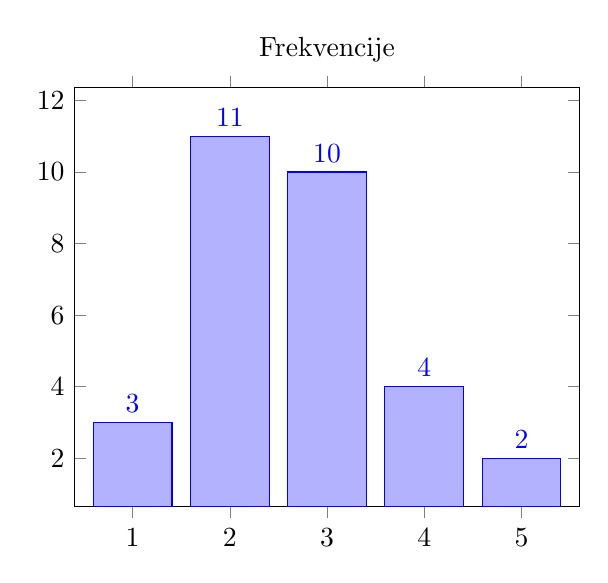
\begin{tikzpicture}
\begin{axis}[
    width=8cm,
    title=Frekvencije,
    ybar,
    legend style={at={(0.5,-0.15)},
      anchor=north,legend columns=-1},
     bar width=1cm, 
    enlargelimits=0.15,
   % ylabel={frekvencije},
    symbolic x coords={1,2,3,4,5},
    xtick=data,
    nodes near coords,
    nodes near coords align={vertical},
    ]
\addplot coordinates {(1,3) (2,11) (3,10) (4,4) (5,2)};
%\legend{ocjene}
\end{axis}
\end{tikzpicture}
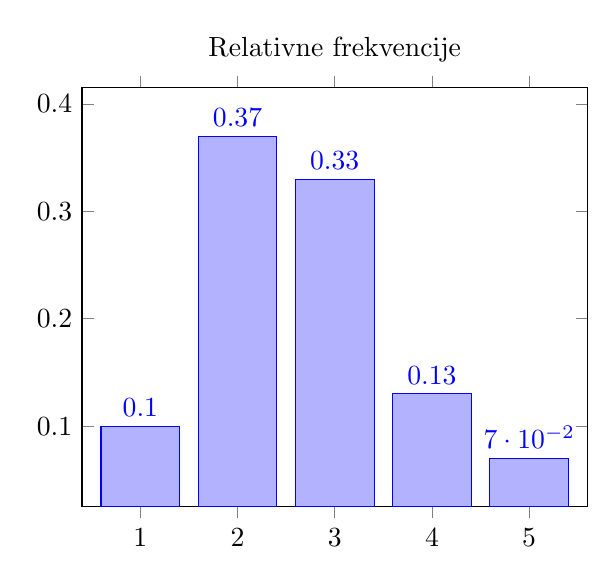
\begin{tikzpicture}
\begin{axis}[
    width=8cm,
    title=Relativne frekvencije,
    ybar,
    legend style={at={(0.5,-0.15)},
      anchor=north,legend columns=-1},
     bar width=1cm, 
    enlargelimits=0.15,
   % ylabel={frekvencije},
    symbolic x coords={1,2,3,4,5},
    xtick=data,
    nodes near coords,
    nodes near coords align={vertical},
    ]
\addplot coordinates {(1,0.10) (2,0.37) (3,0.33) (4,0.13) (5,0.07)};
%\legend{ocjene}
\end{axis}
\end{tikzpicture}
\caption{Stupčasti dijagram frekvencija i relativnih frekvencija}
\label{fig:frekvirelfrekv}
\end{figure}\\
Neka je
\begin{align}
    f_i &:= \#\{\omega\in\Omega:X(\omega)=i\} \\ 
        &\phantom:= \text{frekvencija vrijednosti } i\in\im X\text;\\
    r_i &:= \dfrac{f_i}{n}\label{eq:ri}\\
        &\phantom:= \text{relativna frekvencija od } i\in\im X\text,
\end{align}
gdje je $n=\#\Omega$ \emph{duljina} skupa podataka ($n=30=\text{broj učenika u razredu)}$.

\noindent Izračunajmo frekvencijsku tablicu (tablica~\ref{tbl:frekvencijska}). U prvi stupac zapisujemo vrijednosti ocjena iz matematike (1--5), u drugi stupac pišemo frekvenciju vrijednosti (ocjene) te u treći relativnu frekvenciju ocjene izračunate kao u~\eqref{eq:ri}.
\begin{table}[ht]
\centering
\begin{tabular}{ccc}
\hline
$i$       & $f_i$  & $r_i$ \\ \hline
$1$       & $3$    & $\frac{3}{30}=0.10$ \\
$2$       & $11$   & $\frac{11}{30}\approx 0.37$ \\ 
$3$       & $10$   & $\frac{10}{30}\approx0.33$ \\
$4$       & $4$    & $\frac{4}{30}\approx0.13$ \\
$5$       & $2$    & $\frac{2}{30}\approx0.07$ \\ \hline
$\sum$    & $30$   & $1(\approx1.00)$ \\   \hline
\end{tabular}
\caption{Frekvencijska tablica}
\label{tbl:frekvencijska}
\end{table}
Pomoću frekvencijske tablice nacrtajmo \emph{stupčasti dijagram} frekvencija i/ili relativnih frekvencija (slika~\ref{fig:frekvirelfrekv}). Vidimo da stupčasti dijagrami zapravo izgledaju isto. Dakle, svejedno nam je hoćemo li kod crtanja dijagrama koristiti frekvencije ili relativne frekvencije. Mi ćemo uglavnom crtati dijagrame pomoću relativnih frekvencija.
\end{primjer}
%
\begin{primjer}
Rezultati prodaje ljetnih majica tijekom tri ljetna mjeseca prikazani su frekvencijskom tablicom:
\begin{center}
\begin{tabular}{ccc}
\hline
veličina & frekvencija & relativna frekvencija \\ \hline
S        & $9$         & $0.16$                \\
M        & $30$        & $0.55$                \\
L        & $16$        & $0.29$                \\ \hline
$\sum$   & $55$        & $1.00$                \\ \hline
\end{tabular}
\end{center}
$X=\text{"veličina majice"}$, $\im X=\{S,M,L\}$.
Prikažimo podatke o veličinama majica pomoću \emph{strukturnog dijagrama} (slika~\ref{fig:struktdij}).
\begin{figure}[ht]
    \centering
    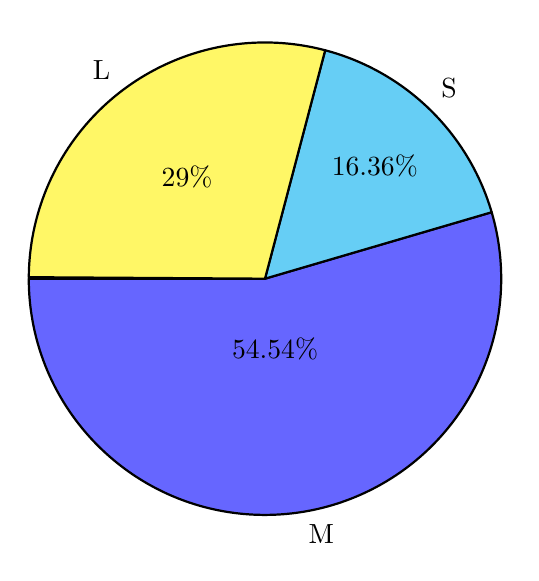
\begin{tikzpicture}
    \pie [rotate = 180]
    {54.54/M,
     16.36/S, 29/L}
    \end{tikzpicture}
    \caption{Strukturni dijagram}
    \label{fig:struktdij}
\end{figure}
\end{primjer}
\section{Zadaci}
Osnovne pojmove potrebne za rješavanje i razumijevanje zadataka možete pogledati u~\cite{predavanja}.
\begin{zadatak}
Kocku smo bacali 20 puta i zabilježili smo sljedeće rezultate:
\begin{center}
\begin{tabular}{cccccccccc}
6 & 3 & 3 & 6 & 3 & 5 & 6 & 1 & 4 & 6 \\
3 & 5 & 5 & 2 & 2 & 2 & 2 & 3 & 2 & 3
\end{tabular}
\end{center}
\begin{enumerate}[(a)]
    \item Nacrtajte histogram relativnih frekvencija.
    \item Odredite aritmetičku sredinu, mod i medijan uzorka.
    \item Odredite varijancu i standardnu devijaciju uzorka.
    \item  Odredite raspon uzorka.
    \item Odredite donji i gornji kvartil te interkvartil uzorka.
    \item Nacrtajte dijagram pravokutnika (\textsl{box and whisker plot}).
\end{enumerate}
\end{zadatak}
\begin{rjesenje}
\begin{enumerate}[(a)]
\item Frekvencijska tablica: tablica~\ref{tbl:frekvtablzad},
\begin{table}[ht]
\centering
\begin{tabular}{c|c|c|c}
$i$    & $y_i$ & $f_i$ & $r_i=f_i/20$ \\ \hline
$1$    & $1$   & $1$   & $0.05$       \\
$2$    & $2$   & $5$   & $0.25$       \\
$3$    & $3$   & $6$   & $0.3$        \\
$4$    & $4$   & $1$   & $0.05$       \\
$5$    & $5$   & $3$   & $0.15$       \\
$6$    & $6$   & $4$   & $0.2$        \\ \hline
$\sum$ &       & $20$  & $1.00$      
\end{tabular}
\caption{Frekvencijska tablica}
\label{tbl:frekvtablzad}
\end{table}
histogram relativnih frekvencija: slika~\ref{fig:histrelfrekvzad}.
\begin{figure}
    \centering
    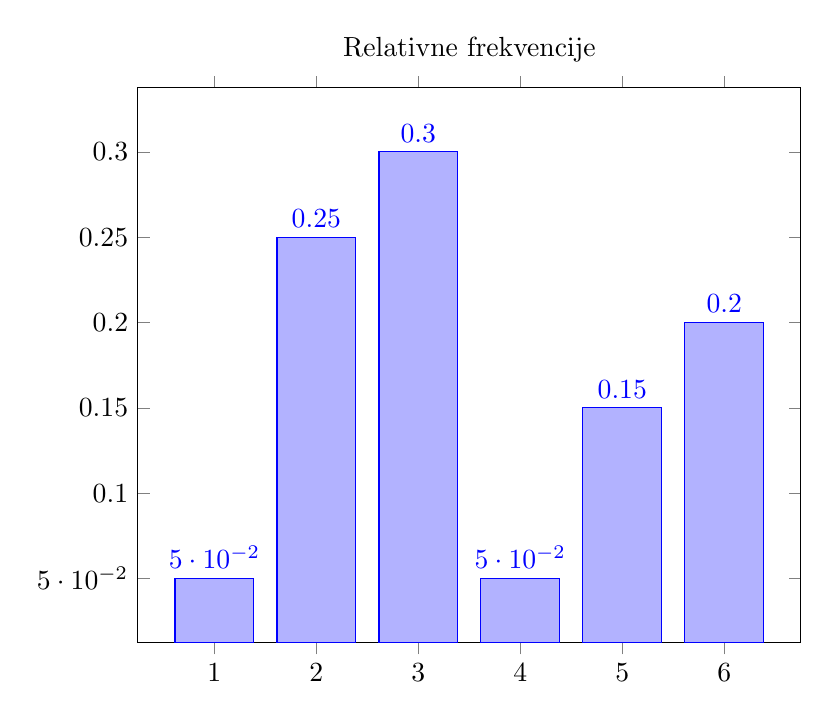
\begin{tikzpicture}
    \begin{axis}[
    width=10cm,
    title=Relativne frekvencije,
    ybar,
    legend style={at={(0.5,-0.15)},
      anchor=north,legend columns=-1},
     bar width=1cm, 
    enlargelimits=0.15,
   % ylabel={frekvencije},
    symbolic x coords={1,2,3,4,5,6},
    xtick=data,
    nodes near coords,
    nodes near coords align={vertical},
    ]
\addplot coordinates {(1,0.05) (2,0.25) (3,0.3) (4,0.05) (5,0.15) (6,0.2)};
%\legend{ocjene}
\end{axis}
\end{tikzpicture}
    \caption{Histogram relativnih frekvencija}
    \label{fig:histrelfrekvzad}
\end{figure}
\item Aritmetička sredina iznosi
\begin{equation}
    \bar{x}=\dfrac{f_1y_1+\cdots+f_6y_6}{f_1+\cdots+f_6}=
    \dfrac{1\cdot1+5\cdot2+6\cdot3+1\cdot4+3\cdot5+4\cdot6}{1+5+6+1+3+4}=3.6
\end{equation}
Mod uzorka je $3$. \\
Podatke $x_1,\dotsc,x_n$ poredane po veličini označavamo s $x_{(1)},\dotsc,x_{(n)}$. Pri tome za $s=k+r$, gdje je $k\in \mathbb{Z}$,$r\in \left[0,1\right>$, vrijedi formula
\begin{equation}
    x_{(s)}=x_{(k)}+r\left[x_{(k+1)}-x_{(k)}\right]\text.
\end{equation}
Medijan uzorka je
\begin{equation}
    m=x_{\left(\frac{n+1}{2}\right)}=x_{\left(\frac{20+1}{2}\right)}=x_{\left(10+\frac{1}{2}\right)}=x_{\left(10\right)}+\dfrac{1}{2}\left[x_{(11)}-x_{(10)}\right]=3+\dfrac{1}{2}(3-3)=3\text.
\end{equation}
\item Varijanca uzorka iznosi
\begin{equation}
    s^2=\dfrac{1\cdot1^2+5\cdot2^2+6\cdot3^2+1\cdot4^2+3\cdot5^2+4\cdot6^2-20\cdot3.6^2}{1+5+6+1+3+4-1}=2.673684
\end{equation}
pa je standardna devijacija $s=1.64$.
\item Raspon uzorka je $R=x_{(20)}-x_{(1)}=6-1=5$.
\item Donji kvartil je
\begin{equation}
    q_L=x_{\left(\frac{n+1}{4}\right)}=x_{\left(\frac{20+1}{4}\right)}=x_{\left(5+\frac{1}{4}\right)}=x_{(5)}+\dfrac{1}{4}\left[x_{(6)}-x_{(5)}\right]=2+\dfrac{1}{4}(2-2)=2\text.
\end{equation}
Gornji kvartil je
\begin{equation}
    q_U=x_{\left(\frac{3(n+1)}{4}\right)}=x_{\left(\frac{3(20+1)}{4}\right)}=x_{\left(15+\frac{3}{4}\right)}=x_{(15)}+\dfrac{3}{4}\left[x_{(16)}-x_{(15)}\right]=5+\dfrac{3}{4}(5-5)=5\text.
\end{equation}
Interkvartil iznosi $d_q=q_U-q_L=5-2=3$
\item Dijagram pravokutnika: slika~\ref{fig:boxplotprvi}.
\begin{figure}
    \centering
    \begin{tikzpicture}
  \begin{axis}
    [
    xtick={},
    xticklabels={},
    boxplot/draw direction=y,
    ]
    \addplot+[
    boxplot prepared={
      median=3,
      upper quartile=5,
      lower quartile=2,
      upper whisker=6,
      lower whisker=1
    },
    ] coordinates {};
  \end{axis}
\end{tikzpicture}
    \caption{Dijagram pravokutnika}
    \label{fig:boxplotprvi}
\end{figure}
\end{enumerate}
\end{rjesenje}
\begin{napomena}
$\left(x_{(1)},q_L,m,q_U,x_{(n)}\right)$ se zove \textsl{karakteristična petorka uzorka}.
\end{napomena}
\begin{napomena}
 Pri formiranju dijagrama pravokutnika \textsl{outlieri} su sve vrijednosti koje su od donjeg ili gornjeg kvartila udaljene za više od $\frac{3}{2}d_q$. \emph{Brkovi} su najmanja i najveća vrijednost koje nisu \textsl{outlieri}. \textsl{Outlieri} se posebno naznačavaju na dijagramu pravokutnika
\end{napomena}
\noindent Primijetite da u prethodnom zadatku nema \textsl{outliera}.
\begin{zadatak}
Na nekom fakultetu je odabran uzorak od $40$ studenata i izmjerene su im visine:
\begin{center}
\begin{tabular}{llllllll}
140 & 188 & 175 & 176 & 177 & 168 & 162 & 181 \\
183 & 187 & 187 & 162 & 184 & 161 & 188 & 169 \\
195 & 171 & 170 & 199 & 181 & 169 & 189 & 191 \\
172 & 182 & 183 & 178 & 180 & 165 & 185 & 205 \\
183 & 187 & 188 & 182 & 163 & 179 & 178 & 188
\end{tabular}
\end{center}

\begin{enumerate}[(a)]
    \item Odredite karakterističnu petorku uzorka.
    \item Nacrtajte dijagram pravokutnika.
\end{enumerate}
\end{zadatak}
\begin{rjesenje}
\begin{enumerate}[(a)]
    \item Gledamo uređene podatke (tablica~\ref{tbl:urpodaci}).
\begin{table}[ht]
\centering
\begin{tabular}{llllllll}
140 & 161 & 162 & 162 & 163 & 165 & 168 & 169 \\
169 & 170 & 171 & 172 & 175 & 176 & 177 & 178 \\
178 & 179 & 180 & 181 & 181 & 182 & 182 & 183 \\
183 & 183 & 184 & 185 & 187 & 187 & 187 & 188 \\
188 & 188 & 188 & 189 & 191 & 195 & 199 & 205
\end{tabular}
\caption{Uređeni podaci}
\label{tbl:urpodaci}
\end{table}
Tada je
\begin{align}
    &n=40\text, \\
    &x_{(1)}=140\text, \\
    &\begin{aligned}
    q_L&=x_{\left(\frac{40+1}{4}\right)}=x_{\left(10+\frac{1}{4}\right)}=x_{(10)}+\dfrac{1}{4}\left[x_{(11)}-x_{(10)}\right]\\
    &=170+\dfrac{1}{4}(171-170)=170.25\text,\\
    \end{aligned}\\
    &\begin{aligned}
    m&=x_{\left(\frac{40+1}{2}\right)}=x_{\left(20+\frac{1}{2}\right)}=x_{(20)}+\dfrac{1}{2}\left[x_{(21)}-x_{(20)}\right]\\
    &=180+\dfrac{1}{2}(181-180)=185.5\text,\\
    \end{aligned}\\
    &\begin{aligned}
    q_U&=x_{\left(\frac{3(40+1)}{4}\right)}=x_{\left(30+\frac{3}{4}\right)}=x_{(30)}+\dfrac{3}{4}\left[x_{(31)}-x_{(30)}\right]\\
    &=187+\dfrac{3}{4}(187-187)=187\text,\\
    \end{aligned}\\
    &x_{(40)}=205\text.
\end{align}
Karakteristična petorka je $\left(140,170.25,180.5,187,250\right)$.
\item Interkvantil iznosi $d_q=q_U-q_L=187-170.25=16.75$ pa je
\begin{gather}
    q_L-\dfrac{3}{2}d_q=145.125\text, \\ q_U+\dfrac{3}{2}d_q=212.125\text.
\end{gather}
Dijagram pravokutnika: slika~\ref{fig:boxplotdrugi}.
\begin{figure}[!ht]
    \centering
    \begin{tikzpicture}
  \begin{axis}
    [
    xtick={},
    xticklabels={},
    boxplot/draw direction=y,
    ]
    \addplot+[mark = diamond,
    boxplot prepared={
      median=185.5,
      upper quartile=187,
      lower quartile=170.25,
      upper whisker=205,
      lower whisker=161
    },
    ] coordinates {(0,140)};
  \end{axis}
\end{tikzpicture}
    \caption{Dijagram pravokutnika}
    \label{fig:boxplotdrugi}
\end{figure}
\end{enumerate}
\end{rjesenje}
\nocite{vjezbe}
\printbibliography
\listoffigures
\listoftables
\end{document}
